Главное окно состоит всего из двух кнопок: <<Монитор>> и <<Настройки>>.
По нажатию на кнопку <<Настройки>>, открывается окно настроек, где возможно изменять настройки программы, 
а также настраивать подключенные к компьютеру считыватели. 

Окно монитора позволяет просматривать информацию
о новых событиях в табличном виде, а также проводить поиск по этой информации. В окне монитора
можно сохранить отфильтрованные данные о событиях в отчет, который затем можно открыть в Microsoft Office 
Excel и распечатать при необходимости.

\begin{center}
    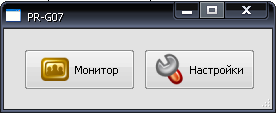
\includegraphics{img/main.png}
\end{center}

